\begin{frame}{\secname : Integer-Pointer casting in C}

  \comment{Example}
  \vfill
  \begin{alertblock}{ISO C Standard}
  \end{alertblock}
  \vfill
  \begin{exampleblock}{Uses}
  \end{exampleblock}
  
\end{frame}

\begin{frame}{Giving semantics to Integer-Pointer Casts in C}

  \comment{A new memory model with semantics and optimizations}\\
  \comment{Reference the paper}\\
  \comment{The benefits of giving semantics to cast}
  
\end{frame}


\begin{frame}{CompCert: a certified C compiler}

  \begin{block}{CompCert}
    \begin{itemize}
      \item From C to ASM (x86, powerpc or arm).
      \item Most passes are proved in Coq.
      \item Supports most of the ISO-C-99 standard.
    \end{itemize}
  \end{block}
  \vfill
  \begin{center}
    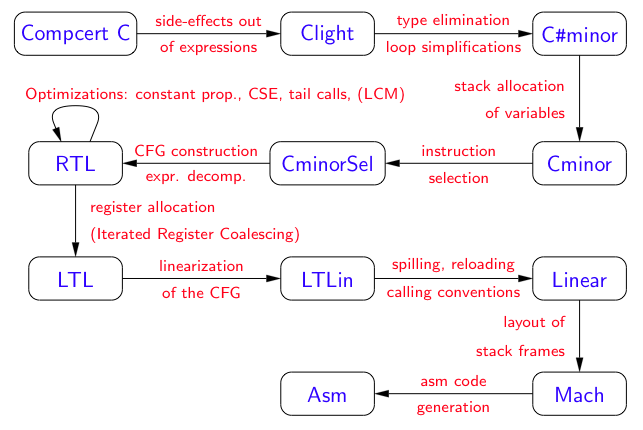
\includegraphics[scale=0.6]{img/passes.png}
  \end{center}
  
\end{frame}


\begin{frame}{Aim of this work}
  
  \begin{block}{Goals}
    \begin{itemize}
    \item Implement the new memory model in CompCert.
    \item Prove the correctness of compilation with this new model.
    \end{itemize}
  \end{block}
  \vfill
  \begin{exampleblock}{Benefits}
    \begin{itemize}
    \item Relevance and usability of the new memory model and semantics.
    \item Allow CompCert to compile correctly a bigger set of C programs.
    \end{itemize}
  \end{exampleblock}

\end{frame}
